%!TEX root = ../../thesis.tex
\renewcommand{\chapterpath}{\allchapterspath/introduction}
\renewcommand{\imgpath}{\chapterpath/img}

\chapter{Introduction}
\label{chapter:introduction}
\minitoc

From robotic vacuum cleaners to self-driving car, smart home thermostat to autonomous trading, more and more autonomous intelligent systems are coming into our daily life, taking on their own decisions that can affect our everyday life. As such system becomes more and more advance and intricate, they also become more and more difficult to predict. As a direct consequence, it will be more and more difficult to explicitly get them to do what we want them to do. Their internal mechanisms can no longer be understood by a single person which makes the need to integrate simple, intuitive, and high-level interacting capabilities to those systems primordial.

We start by providing a small vision of what autonomous intelligent systems are nowadays and then present a brief overview of the main challenges involved when designing autonomous systems. We further explicit the need for such system to learn from their environment and present the major learning paradigms used nowadays. After focusing our analysis on learning paradigms based on interaction with human, we introduce the recent advances in interactive learning where the human and the learning system are in close interaction. Finally we identify and introduce the problem of interacting with a system without pre-coordination of communicative means. We call this challenge the problem of \textbf{fluid interactive learning} which is the main topic investigated in this thesis.

Most of our discussions will be articulated around the current trend of autonomous robots that are predicted to play an important role into our daily life in the coming century. However we would like the reader to keep in mind that an autonomous intelligent interactive system, such as a robot, can take many other form such as a virtual agent, a smartphone, or an intelligent prosthesis.

%%%%%%%%%%%%%%%%%%%%%%%%%%%%%%%%%%%%%%%%%%%%%%
%%%%%%%%%%%%%%%%%%%%%%%%%%%%%%%%%%%%%%%%%%%%%%
%%%%%%%%%%%%%%%%%%%%%%%%%%%%%%%%%%%%%%%%%%%%%%
%%%%%%%%%%%%%%%%%%%%%%%%%%%%%%%%%%%%%%%%%%%%%%
%%%%%%%%%%%%%%%%%%%%%%%%%%%%%%%%%%%%%%%%%%%%%%
\section{Autonomous intelligent systems around}

At home, workplaces or schools, an increasing amount of intelligent robotic systems are starting to be able to help us in our daily life (windows or vacuum cleaners, self-driving cars) \cite{gates2007robot} and in flexible manufacturing systems \cite{baxter} (Figure~\ref{fig:introduction:robots}). They are characterized by their ability to take important decisions autonomously, such as whether or not to engage at crowded road crossing. It is very different from the usual protective fences in industrial robots which creates several challenges related to safety, unpredictable environments, acceptability and usability by and adaptation to non-technically trained people. 

Most of the autonomous intelligent systems are developed with the aim to improve users quality of life and should therefore comply to the preferences of each users. My autonomous car should come take me at work at 6 p.m. and bring me back home. My vacuum cleaner should vacuum only the rooms I want at the time of the day I decided. My smart watch or smart glass should display the information that matters to me. My surveillance robot should patrol around my house following the specific pattern I envision.

\begin{figure}[!h]
    \centering
    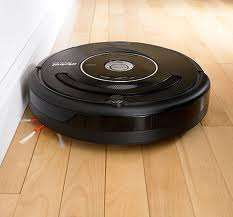
\includegraphics[height=0.2\columnwidth]{\imgpath/roomba.jpg}
    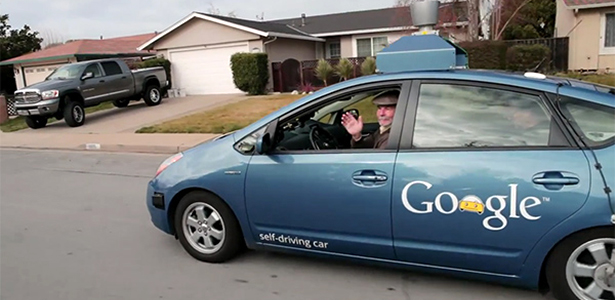
\includegraphics[height=0.2\columnwidth]{\imgpath/google_self_driving_car.jpg}
    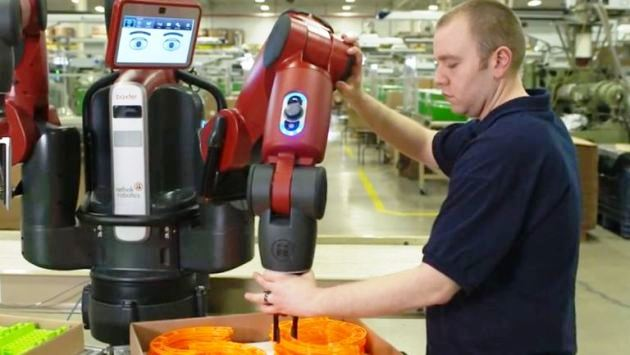
\includegraphics[height=0.2\columnwidth]{\imgpath/baxter_coworking.jpg}
    \caption{Three examples of nowadays autonomous intelligent robots. From left to right: a Roomba vacuum cleaner, an autonomous car from Google, and a collaborative robotic worker called Baxter.}
    \label{fig:introduction:robots}
\end{figure}

How can we balance autonomy and commitment in autonomous intelligent systems? In order to have machine performs complex task for us, that require complex sensing, acting and planning skills we need to endow them with the ability to make plans and learn from their day to day experience. Once such system as the ability to perform many different tasks in many different ways, the question of how to explicitly get these robots to do what we want becomes of crucial importance. The following section briefly introduce the many challenges associated to the design of autonomous intelligent machines.

%%%%%%%%%%%%%%%%%%%%%%%%%%%%%%%%%%%%%%%%%%%%%%
%%%%%%%%%%%%%%%%%%%%%%%%%%%%%%%%%%%%%%%%%%%%%%
%%%%%%%%%%%%%%%%%%%%%%%%%%%%%%%%%%%%%%%%%%%%%%
%%%%%%%%%%%%%%%%%%%%%%%%%%%%%%%%%%%%%%%%%%%%%%
%%%%%%%%%%%%%%%%%%%%%%%%%%%%%%%%%%%%%%%%%%%%%%
\section{Challenges}

As robots enter more and more into our daily life they will have to deal with our daily environment that is often unstructured and open-ended. In this section we identify and briefly present six main challenges of nowadays robotics: sensing, acting and planning, social interaction, morphology, adaptation and life long learning.

\subsection{Sensing and analyzing}

\question{How can a robot sense and make sense of its environment?}

Sensing start by developing advance sensors allowing the robot to collect information about the relevant features of its environment. Most of the work on sensor applied to robotic lies in vision and localization systems which are primordial for the robot to known where object are in the environment and where the robot it-self is in that environment. But having access to a raw image do not give the robot the ability to locate in a room. Some analysis of the raw sensors information is required to recognize objects in a scene \cite{filliat2007visual}, people in a room \cite{nakauchi2002social}, or the robot location \cite{durrant2006simultaneous, bailey2006simultaneous} and also to understand facial expression \cite{valstar2006fully}, gesture \cite{nickel2007visual} or gaze direction \cite{matsumoto2000algorithm}.

This problem is inherent to most of the modalities used in robotics nowadays. From sounds waves, robots may need to infer the location of speaker \cite{nakadai2002real,valin2003robust}, the recognition of a pronounced word \cite{rabiner1989tutorial}, and the emotional state of the speaker \cite{oudeyer2003production}. From touch, they should the texture \cite{howe1989sensing,nguyen2011texture}, hardness \cite{shikida2003active} or shape \cite{schneider2009object} of an object, avoid too strong impacts \cite{alami2006safe} , and even dose their physical contact with human \cite{nakagawa2011effect,miyashita2007haptic}. And from raw millimeter precision Lidar sensors, they should identify pedestrian, bicycle, car, truck position and their intention \cite{himmelsbach2008lidar}. In addition information from different sensors can be merge together to gain access to new kinds of information or gain precision in one specific estimate \cite{xiong2002multi}. 

However having access to high level and precise information from the environment is useless for a robot if it can not be used to act appropriately in the environment.

\subsection{Acting and planning}

\question{How can a robot affect its environment and plan its actions in our cluttered and dynamics environment?}

Acting starts by developing advance actuators allowing the robot to alter the current state of its environment. Most of our robot actuators today are motor based and produce many forms of motion from rotary movements. However being able to produce movements does not mean the robot will produce useful movements. As sensing requires analyzing, acting requires planning.

A robot that should evolve in our daily life should be able to move around our houses where many objects are constantly changing positions, with stairs, different floor's types and even human and animals moving around. Assuming the robot can sense and analyze every information needed to navigate, it still need to coordinate all its actuators in order to reach a goal. This coordination problem is especially difficult for problem like walking \cite{kajita20013d,lapeyre2011maturational} or grasping \cite{bicchi2000robotic} where many degrees of freedom are involved and should be synchronized in a proper way.

Acting is often an integral part of the sensing process, where sensors like cameras are mounted on articulated pan-tilt actuators to mimic human eyes. In this case the act of sensing is tightly coupled with the act of moving \cite{bajcsy1988active,lonini2013robust}.

\subsection{Interacting with social peers}

\question{How can a robot interact and communicate with humans?}

As robots are meant to help us in our daily life, they need to be able to interact with us, to understand us and be understood by us. To be understood a robot should act in a socially acceptable manner, adapt its behavior to the current context of interaction, express its current state by displaying familiar signs of emotion using on the appropriate modality.

Being social is also reacting correctly to the social signals sent by the other social beings. It requires the robot to sense and analyze touch, speech, gestures, gaze, facial expression, or other kinds of interfaces but also normative social rules such as appropriate distance of interaction \cite{strait2014let}, eye contact \cite{andrist2014conversational}, hand over \cite{moon2014meet}, or trajectory \cite{kruse2014evaluating} dynamics.

This multi-disciplinary study of social interaction between human and robot is the field of human-robot interaction (HRI) \cite{fong2003survey,dautenhahn2007socially,goodrich2007human}. An important challenge is to design and conduct human-robot interaction studies which allow to evaluate the objective and subjective usability and acceptability of the human-robot interaction \cite{scholtz2003theory,walters2005practical,young2011evaluating}.

\subsection{Design, morphology and appearance}

\question{What geometry, color, size, or shape should take a robot to be socially accepted among humans as well as efficient in its everyday activities?}

The morphology and appearance of a robot are properties that impacts all the previously defined challenges. The way the different parts of the body are design will affect the ease of the robot to perform a daily task. The way a sensor is located on its body will affect the sensing performance and its analysis. And the way a robot looks will affect its ability to tight up link with surrounding human could make the more technology advance robot worthless. We will highlight the influence of morphology and appearance for acting, sensing, and socially interacting using three using concrete example from the literature.

\paragraph{Better acting} The geometry and distribution of mass in the body has complex influences on biped locomotion. Several studies have for example explored the role of the foot and ankle morphology for biped walking on both human and robot, but the impact of various thigh shapes a robot dynamics \cite{lapeyre2013poppy}. This later work study the impact of a bio-inspired thigh, bended of 6 degree and with a geometry inspired by humans, on the balance and biped locomotion compared to a more traditional straight thigh. They have shown that the bio-inspired thigh allows the reduction of falling speed by almost 60\% and the decrease of the lateral motion needed for the mass transfer from one foot to the other by 30\%.

\paragraph{Better sensing} The design component of the body is also important for the sensing capabilities of the robot. As an example, the fingerprint while moving our finger on a textured surface enhance our ability to differentiate textures \cite{hollins2010somesthetic} compared to a smooth finger surface. By taking inspiration from the fingerprint properties, researcher have created an artificial finger that is more sensitive to textured surface \cite{candelier2011role}.

\paragraph{Better acceptability}

Effect of robot appearance on human-robot interaction is a widely investigated topic \cite{li2010cross, heerink2006studying}. One of its prominent characteristic is called the uncanny valley \cite{mori1970uncanny}, which state that the relation between human likeness of a robot and its perceived familiarity by human does not hold a linear relation. It states that familiarity increases with human likeness until a point is reached where a subtle deviations from human appearance and behavior create a unnerving effect, which is called the uncanny valley. More recent developments speculate that maybe even the most human-like androids, and even real human faces, are not liked as much as toy robots or humanoids. This effect has been called the uncanny cliff \cite{bartneck2007uncanny}.

\subsection{Adapt, adapt, adapt}

\question{How can a robot adapt to our open ended and dynamics environment \\ throughout its lifetime?}

Things change and a robot that is designed, built and programmed to live in todays words will have to learn new skills during his life time. It may even have to learn them right from the beginning, such as learning the language and habits of the community it leaves in. It may also break some of its parts, and will have to learn to deal with it or to adapt to the properties of the new replacement parts.

Therefore rather than trying to represent all human knowledge in our robots it seems more natural to endow them with the ability to learn. This idea has been formulated more than sixty years ago by Alan Turing \cite{turing1950computing} advocating that ``instead of trying to produce a programme to simulate the adult mind, why not rather try to produce one which simulates the child's?''. 
This precise line of research really began to be explored in the beginning of the century with the emerging field of developmental robotics \cite{weng2001autonomous,lungarella2003developmental} which ``aims at studying the developmental mechanisms, architectures and constraints that allow life long and open-ended learning of new skills and new knowledge in embodied machines'' \cite{oudeyer2012developmental}. 

While the idea of learning for machine is commonly accepted, developmental robotics is yet an emerging field inside the robotic and machine learning community. Most of the learning algorithm today do not take into account many aspects of the real life challenges robot should be able to face in our open-ended and dynamic environment. 

\paragraph{Open-ended environment} Most of the learning literature focus on abstract and well structure problems, where the researcher define in advance a representation well suited to the problem. But not every problem can be define in advance, as we learn to use smartphone which did not exist few years back, a robot should be able to learn how to use new systems without the need for an engineer to reprogram it, and this throughout their life time.

\paragraph{Lifelong learning} Lifelong learning can be define as the ongoing and self-motivated pursuit of knowledge and the ability needed to adapt to our everyday problems. Most of the learning literature do not consider learning as an ongoing activity. As an example, classification algorithms often need to have access to a batch of labeled examples which must therefore be collected by an engineer beforehand. But in order to adapt to our everyday problems embodied autonomous robots should be able to actively seek and select useful information in their environment. 

% maturational constraints biasing and constraining learning process

In the next section we describe the three main learning paradigms considered nowadays: learning from extrinsic motivation, intrinsic motivation, and social interaction.

%%%%%%%%%%%%%%%%%%%%%%%%%%%%%%%%%%%%%%%%%%%%%%
%%%%%%%%%%%%%%%%%%%%%%%%%%%%%%%%%%%%%%%%%%%%%%
%%%%%%%%%%%%%%%%%%%%%%%%%%%%%%%%%%%%%%%%%%%%%%
%%%%%%%%%%%%%%%%%%%%%%%%%%%%%%%%%%%%%%%%%%%%%%
%%%%%%%%%%%%%%%%%%%%%%%%%%%%%%%%%%%%%%%%%%%%%%
\section{Learning paradigms}

Hard coding control or planning solutions into robots is not a viable solution for robots that aims at entering into our daily life. Learning seems to be a more promising approach and many work have tackled this problem. Among them we can draw three main paradigms: \begin{inparaenum}[(a)] \item learning from extrinsic motivation, where an objective is given to the robot that should be either maximize or minimize \item learning from intrinsic motivation, where the robot define its own objectives, and \item social learning, where a social agent which as already acquired some skills helps an other agent to acquired the same skills, it is characterized by a tight interaction loop between the two partners. \end{inparaenum}. The following subsections provide a small introduction to the three paradigms.

\subsection{Learning from human defined objective function: extrinsic motivation}

Extrinsic motivations are driven by external rewards or punishments which arise from outside of the robot own control. It is a measure of fitness with respect to a given objective. For robots, these functions are usually defined by the engineer and the role of the learning system is learn to optimize them using its acting possibilities. It can be a hard-coded pain like punishment useful for the robot to learn to avoid braking itself, or a reward proportional to the position shift of the robot with respect to a predefined path to follow, or a boolean stating if a task is correctly executed or not.

the robot does the job and explore
Well known results include hand writing recognition, scene analysis on the perceptual learning side and on the task learning side. some robot example.
reinforcement learning


\subsection{Self-directed learning: intrinsic motivation}

Intrinsic motivations are driven by an interest in the activities for their own sake which arises from within the robot and depends on its own internal operations rather than on external pressures or rewards. Intrinsic motivations allow the robot to gain autonomy with respect to the open-ended challenges it may face into the real words. 

As for extrinsic motivation the robot does the job and explore

\subsection{Learning from others: social interaction}



the robotis guided


%
In particular, such robotic systems need to be teachable by non-technical users, i.e. \textbf{programmable for new tasks in novel environments} through \textbf{intuitive, flexible and personalized interactions}. Specifically, the challenge we address in this work is how a robot learning a new task can be instructed by a human using its own preferred teaching signals, where the mapping between these signals and their meaning may be initially partially or even totally unknown to the robot (e.g. a user may use a different language, words, interjections or gestures to mean ``good'' or ``bad'' or ``turn left'').



The categorization of learning paradigms above in three categories does not reflect the many subfamilies that exist between these categories, including those that are shared among categories. It is meant to situate the learning problem into a more global picture, providing some interesting pointers for the interested readers. 

This thesis focus on the social learning aspects, where robots should learn by observing or being instructed by a human. Next section provide more details of the social learning literature, which we organized in three main groups: learning from human demonstrations, learning from human reinforcement, and learning from human instructions. 

%%%%%%%%%%%%%%%%%%%%%%%%%%%%%%%%%%%%%%%%%%%%%%
%%%%%%%%%%%%%%%%%%%%%%%%%%%%%%%%%%%%%%%%%%%%%%
%%%%%%%%%%%%%%%%%%%%%%%%%%%%%%%%%%%%%%%%%%%%%%
%%%%%%%%%%%%%%%%%%%%%%%%%%%%%%%%%%%%%%%%%%%%%%
%%%%%%%%%%%%%%%%%%%%%%%%%%%%%%%%%%%%%%%%%%%%%%
\section{Robot Learning from Humans}


Next section provide more details of the social learning literature, which we organized in three main groups: learning from human demonstrations, learning from human reinforcement, and learning from human instructions. 

When who what when to imitate?

Research in robotics has long been inspired by human social learning. Among other aspects, learning by demonstration/imitation has attracted the most attention. It has provided several examples of efficient learning in robotic systems \cite{argall09survey,lopes10imitationchapter}. Data from a human teacher has been used as: initial condition for further self-exploration in robotics \cite{nicolescu2003natural}, bootstrapping further intrinsically motivated learning \cite{nguyen2011bootstrapping}, information about the task solution \cite{calinon07}, information about the task representation \cite{macl07affimit}, among others. Several representations have been used to generalize the demonstration data using reinforcement learning \cite{thomaz2008teachable}, inverse reinforcement learning \cite{macl07affimit,Abbeel04icml} or regression methods \cite{calinon07,chernova09jair}. The different formalisms make use of different information and extract different knowledge, either direct policy information or a reward function that explains the behavior.

\subsection{Learning from human demonstrations}

correspondence problem 

\subsection{Learning from human reinforcement}

\subsection{Learning from human instructions}

lies at the interaction of those domains

The categorization of learning paradigms above in three categories does not reflect the many subfamilies that exist between these categories, including those that are shared among categories. It is meant to situate the social learning problem in a more global picture, providing some interesting pointers for the interested readers. 

As we noticed, in most of the above presented work, the human and the robot had no or few well controlled interaction with the robot. The properties of teaching interactions with a human in the loop was not considered in depth. This issues have began to be addressed in a subfield called \emph{interactive learning}  which combine ideas of social learning its different forms with extrinsic and intrinsic motivated learning. Where the robot acquire a form of autonomy with respect to how to deal with the human in the loop. This leaded to interesting results concerning the behavior of human in such situation.

%%%%%%%%%%%%%%%%%%%%%%%%%%%%%%%%%%%%%%%%%%%%%%
%%%%%%%%%%%%%%%%%%%%%%%%%%%%%%%%%%%%%%%%%%%%%%
%%%%%%%%%%%%%%%%%%%%%%%%%%%%%%%%%%%%%%%%%%%%%%
%%%%%%%%%%%%%%%%%%%%%%%%%%%%%%%%%%%%%%%%%%%%%%
%%%%%%%%%%%%%%%%%%%%%%%%%%%%%%%%%%%%%%%%%%%%%%
\section{Interactive Learning}

demonstration, human generated reward

Perceptual learning and task learning can both benefit from user interaction in many different ways. On the one hand, if the interaction protocol and context, is well defined it is possible to acquired grounded perceptual data. On the other hand, if the human and the machine understand each others, the human can explain or guide the machine, which may reduce learning time or even enable the machine to learn task difficult to write down as an objective or reward function.


People will not always respect predefined conventions. Several studies discuss the different behaviors naive teachers use when instructing robots \cite{thomaz2008teachable,Cakmak2010optimality}. An important aspect is that the feedback is frequently ambiguous and deviates from the mathematical interpretation of a reward or a sample from a policy. For instance, in the work of \cite{thomaz2008teachable} the teachers frequently gave a positive reward for exploratory actions even if the signal was used by the learner as a standard reward. Also, even if we can define an optimal teaching sequence, humans do not necessarily behave according to those strategies \cite{Cakmak2010optimality}. For more studies on how humans teach robots see \cite{thomaz2009learning,kaochar2011towards,knox2012humans}. These studies show that even when using well defined protocols, it is important to consider how different instructions can be used for learning. 

Nevertheless the real problem is somewhat even more complicated. Figure shows this complexity. When observing the robot behavior the user will provide some instructions, using vocal commands for instance. If their meanings are known and the speech recognition system works then they can be directly translated into learning data for the task learning algorithms. But in general, it is important to consider that there can be errors in the recognition system, even systematic when taking into account accents, and that people might be more comfortable to use different, not predefined, words. The problem now becomes that the meaning of these new instructions can not be easily recovered if the task that is being learned is not known.

However most of those systems have not considered in depth the properties of teaching interactions with a human in the loop. The demonstrations are provided in a batch perspective where data acquisition is done before the learning phase. Those issues have began to be addressed in works studying \textit{interactive learning} \cite{kaplan2002robotic,nicolescu2003natural,Breazeal2004,thomaz2008teachable}, which combines the ideas of learning from demonstration, learning by exploration and tutor feedback. Under this approach, the teacher interacts with the robot and provides extra feedback or guidance. In addition, the robot can act to improve its learning efficiency. Recent developments have considered: extra reinforcement signals \cite{thomaz2008teachable}, action requests \cite{macl09airl}, disambiguation among actions \cite{chernova09jair}, preferences among states \cite{Mason2011}, iterations between practice and user feedback sessions \cite{judah2010reinforcement} and choosing actions that maximize the user feedback \cite{knox2009interactively}.

Interactive learning \cite{nicolescu2003natural,breazeal2004tutelage} aims at developing systems that can learn by practical interaction with the user and finds applications in a wide range of fields such as human-robot interaction, tutoring systems or human-machine interfaces.
This type of learning combines ideas of learning from demonstration \cite{argall09survey}, learning by exploration \cite{thrun1992efficient} and tutor feedback \cite{kaplan2002robotic}. Under this approach the human teacher interacts with the machine and provides extra feedback or guidance. 

In addition, the device can act to improve its learning efficiency.
Approaches have considered: extra reinforcement signals \cite{thomaz2008teachable}, action requests \cite{lopes2009active}, disambiguation among actions \cite{chernova09jair}, preferences among states \cite{Mason2011}, iterations between practice and user feedback sessions \cite{judah2010reinforcement}, and choosing actions that maximize the user feedback \cite{knox2009interactively}. 

\subsection{Online interactive learning}

\subsection{How people teach robots}

\subsection{User modeling and ambiguous protocols}

\cite{macl11simul}

\subsection{Ambiguous signals}

\subsection{Active learner}

\subsection{Active teacher}



find some framework and cite thomas \cite{cederborg2013language}

Perceptual learning and task learning can both benefit from user interaction in many different ways. On the one hand, if the interaction protocol and context, is well defined it is possible to acquired grounded perceptual data. On the other hand, if the human and the machine understand each others, the human can explain or guide the machine, which may reduce learning time or even enable the machine to learn task difficult to write down as an objective or reward function.




This thesis lies around those challenges. We identified one important assumtion made in all those experiments. The facts that the human and the robot are assuemd to be able to undertasn each others on one level or an other before the interaction can begin. Whether the meaning of the social signals are known and the robot should infer the task, or the task is known and the robot should infer some characteristic of its human partners, wheter the mapping between some communicative signals and their meaning, or the frequeccy to which it tends to use some words.

\section{The challenge of fluid interactive learning}



How can a robot learn to interpret our different modes of communication? 

Interactive learning combines the ideas of learning from demonstration, learning by exploration and tutor feedback. Two widely explored subfields are:
\begin{itemize}
\item \textbf{Interactive perceptual learning} in which the system learns to discriminate between perceptual events via the help of a human partner. If the interaction protocol and context is well defined it is possible to acquired grounded perceptual data. It implies \textbf{the machine is aware of the communicative goal of the human}.
\item \textbf{Interactive task learning} in which the system learn to increase its performance with respect to an objective or a reward function via the help of a human partner. If the human and the machine understand each others, the human can explain or guide the system, which may reduce learning time or even enable the machine to learn task difficult to write down as an objective or reward function. Therefore a usual assumption is that \textbf{the machine understands the meanings of human' s  communicative signals}.
\end{itemize}

Their respective assumptions makes those two lines of research incompatible. On the one hand, working on perceptual learning, i.e. learning the signal-to-meaning mapping, requires the machine to know the task. On the other hand, teaching a new task to a machine requires to already know the signal-to-meaning mapping. Consequently it is impossible for a user to instruct --- from scratch --- a machine using his own preferred teaching signals, the user must comply to the use of predefined ones or go through a calibration procedure.

Unknown signals, unknown tasks

A usual assumption in such systems is that the learner and the teacher share a mutual understanding of the meaning of each others' signals, and in particular the learning agent is usually assumed to know how to interpret teaching instructions from the human. In practice, this problem can be solved due to two simplifications. On one hand, the range of accepted instructions is limited to those predefined by the system developer. This approach, commonly used in human-robot interaction, lacks flexibility and adaptation to user specificities and, consequently, may not be well accepted by non-experts users with different preferences. 
%
On the other hand, sometimes it is not enough to predefine the instruction sets and it is necessary to perform a calibration phase to map raw signals such as speech or brain activity to the meaning. This is usually done using an ad-hoc protocol to collect labeled samples of the user communicative signals. This process must be well controlled to ensure signals are associated to the true intended meaning of the user.

The previous engineering solution is needed due to the chicken egg nature of the problem. In order to teach a system a new skill, it needs to understand the human instructions. And, in order to understand this feedback, the system must have some interaction with the human (e.g. through a controlled task as done in the calibration process) to learn what the instructions mean. 

Few works have studied and developed interactive learning systems that can learn both the meaning of symbols and the task simultaneously. In human-robot interaction Griffiths et al. \cite{griffiths2012bottom} conducted an experiment with humans learning the meaning of unknown symbolic teaching signals. Lopes et al. \cite{macl11simul} presented sequential task experiments considering symbolic teaching signals and requiring a bootstrap with known signals. Grizou et al. \cite{grizou2013robot} extended their system for non-symbolic teaching signals while removing the need for bootstrapping with known signals. Non-invasive brain-computer interfaces (BCIs) have also looked at this problem, since they usually require user-dependent calibration and have to deal with the EEG brain signals non-stationarities. These facts, together with the poor signal-to-noise ratio of the EEG, make the EEG self-calibration one of the most challenging ones. Specifically, for P300 spellers, Kindermans et al. have shown that it is possible to exploit the repetition of signals together with prior information  \cite{Kindermans2012a,Kindermans2012b} to calibrate the system while using the speller.


While research on robot learning from human interaction has flourished in the last ten years, most work has focused on how to extract statistical \textit{task models} from human teachers following a fixed pre-defined teaching protocol (e.g. using a pre-defined button for ``good'' or ``bad'' feedback or using ad-hoc words for guidance with a trained speech recognition and dialog system). Thus, a usual assumption is that the learner and the teacher share a mutual understanding of the meaning of each others' instructions, and in particular the robot is usually assumed to know how to interpret instructions from the user. In practice, the range of accepted signals is limited to the one predefined by the system developer. Also, it is often assumed that instructions are noiseless and can be directly used as a feedback signal for a learning algorithm. The question of how a robot can learn to interpret personalized and potentially noisy teaching signals, i.e. learn \textit{instruction models}, has been much less explored.

We can now define a general scientific challenge: \textit{Can a robot learn a new task if the task is unknown and the user is providing unknown instructions? Which are the constraints and mechanisms that could provide this flexibility in interactive task learning?} There are two important dimensions in such questions: 1) which are the computational machine learning algorithms and formalisms that are needed for this goal? 2) how to integrate them within real-world meaningful human-robot interaction such that usability and acceptability can be evaluated in user studies. Given the complexity and novelty of these issues, this article focuses on the first dimension, elaborating a formalism as well as algorithms that have good properties to address the broader challenge. While we present an exepriment with a real robot and discuss the second dimension in the discussion section, more thorough real-world user studies will be achieved in future work. Yet, we believe the theoretical work presented in this article can constitute an important first step towards flexible personalized teaching interfaces, and thus towards what we may call \textbf{fluid interaction learning}, a key for the future of personal robotics.

In the following, we present a system able to learn the meaning of instruction signals provided by a user using unlabeled speech while learning a task using inverse reinforcement learning. Our contributions are:
\begin{itemize}
    \item a learning algorithm that learns how unknown sub-symbolic instructions signals can be translated in a meaningful teaching signal (among a repertoire of possible ones) that can be used for learning a task (within a space of possible tasks);
    \item a learning algorithm that simultaneously learns the meaning of the instructions and a new task;
    \item an extension of uncertainty based planning in the context of IRL;
    \item tests with robotic systems using voice commands provided by a user using different representations: a finite MDP and an MDP with continuous state representation.
\end{itemize}

After detailing the related work in Section, we provide in Sectiondetails on the algorithm for learning tasks from unknown instructions. Section describes a set of experiments, where we will evaluate the algorithm in different settings. Section introduces an uncertainty based planning algorithm for efficient learning and we show the corresponding results in Section. Finally, we will discuss the main limitations of this work and suggest some future lines of research in Section. 


Our approach is based on a discretization of the possible tasks into a finite number. Each task assigns different expected meanings to the instruction provided by the user. The machine solves the most likely task according to a pseudo-likelihood function computed using the corresponding task labels. The experimental results, both synthetic and based on real EEG data, show that in order to simultaneously recover the meanings and solve the task it is of paramount importance to take into account the uncertainty on both task and signal space.

In the following section, we present the set of assumptions and algorithmic details of our system. Then we introduce the specificity of the uncertainty inherent to our problem using an intuitive example and present the details of our action selection method. Finally we present a set of simulated experiment showing that 
\begin{inparaenum}[a)]
\item our action selection method is reliable and improved over other methods
\item our algorithm scale to the use of high dimensional signals coming from previously recorded brain signals
\item by being operational from the first step, as opposed to calibration procedure, we can estimate the correct task as soon as sufficient evidence has been collected.
\end{inparaenum}

This work is particularly relevant for system requiring an individual adaptation to the user. For instance brain-computer interfaces (BCIs) are systems capable of decoding neural activity in real time, thereby allowing a machine to be directly controlled by thought. Such interfaces must be highly customized to adapt to each user brain signals. It often requires a fastidious calibration procedure, where the user is asked to repeat hundreds of time the same thought process in order to collect labeled data used to train a decoder, also called classifier.

\section{Thesis Statement}

In this dissertation, I will advance the following thesis:

\begin{quote}
Under specific conditions, it is possible to start interacting with a device without pre-coordinating on the signals used for communicating meanings neither on what the device should aim for.
\end{quote}

\section{Thesis Outline}

The purpose of this manuscript is to explain the problem of learning from unlabeled instruction and to provide an intuition on how to solve this problem. I will introduce the most important aspects of the work by simple, hopefully intuitive, visualization of the problem and of the specific properties we exploit. My aim is therefore to endow the interested readers to implement their own version of the algorithm with the tools they are more familiar with.

In chapter 2, I will present an overview of the related work which span from language acquisition to brain computer interfaces. 

In chapter 3, I will introduce a new experimental setup to study the co-construction of interaction protocols in asymmetric collaborative tasks with humans. By presenting preliminary results based on this setup, I will derive interesting lessons for our problem. This work on human experiment is a joint collaboration with Anna-Lisa Vollmer and Katharina J. Rohlfing. 

In chapter 4, I will introduce in more specific terms the problem and provide a visual intuition on what properties we will exploit. I will continue by formalizing the problem in a probabilistic framework, describe how particular brick of the problem are implemented and present results from a robotic pick and place scenario.

In chapter 5, I will introduce the problem of planning related to the problem and provide a visual intuition on what properties we should track. I will continue by defining the uncertainty measure used in the planning process and demonstrate on a 2D grid world problem the efficiency of the method with respect to other planning strategies.

In chapter 6, I will present an application of the algorithm to a BCI scenario where a subject control an agent on a grid. We will describe online experiment showing that our algorithm allow our subjects to start controlling the device without any calibration procedure and by mentally assessing the device's actions. This work on BCI is a joint collaboration with I{\~n}aki Iturrate and Luis Montesano.

In chapter 7, I will discuss the limitation of the work and exemplify, using simulated experiments, direction which could be pursue to overcome them.

